%
% LaTeX report template 
%
\documentclass[a4paper,12pt]{article}
\usepackage{graphicx}
\usepackage[english]{babel}
\usepackage{fontspec}
\usepackage{listings}
\usepackage{xcolor}
\usepackage{float}
%
% set python code style
\definecolor{codegreen}{rgb}{0,0.6,0}
\definecolor{codegray}{rgb}{0.5,0.5,0.5}
\definecolor{codepurple}{rgb}{0.58,0,0.82}
\definecolor{backcolour}{rgb}{0.95,0.95,0.92}
\lstdefinestyle{pystyle}{
	backgroundcolor=\color{backcolour},   
	commentstyle=\color{codegreen},
	keywordstyle=\color{magenta},
	numberstyle=\tiny\color{codegray},
	stringstyle=\color{codepurple},
	basicstyle=\ttfamily\footnotesize,
	breakatwhitespace=false,         
	breaklines=true,                 
	captionpos=b,                    
	keepspaces=true,                 
	numbers=left,                    
	numbersep=5pt,                  
	showspaces=false,                
	showstringspaces=false,
	showtabs=false,                  
	tabsize=2
}
\lstset{style=pystyle}
%
%font
\setmainfont{Times New Roman}
%
%figure space
%
\setlength{\abovecaptionskip}{0.cm}
\setlength{\belowcaptionskip}{0.cm}   
%
%
%start document
\begin{document}
%
   \title{\textbf{DSP assignment2 report}}

   \author{Jingyan Wang, 2533494w \\ Qianqian Wang , 2595993w}
          
   \date{}

   \maketitle
   
   \tableofcontents
 
  \newpage
% after a "%" symbol is treated as comment

\section{Task1}
\subsection{}
With the defination of FIR filter:
$$
x(n) = \sum_{i=0}^{ntaps}h(i)x(n-i)
$$
We implemented the FIR filter with buffer defined with:
\begin{lstlisting}[language=Python]
#add a new value to the buffer
self._buffer[self._offset] = v

for indexH in range(self._ntaps):
		# indexH means i and indexX means n-i
		indexX = self._offset - indexH
		if(indexX < 0):
		indexX += self._ntaps     
		output +=self._coefficcients[indexH]*self._buffer[indexX]

self._offset+=1
if self._offset >= self._ntaps:
		self._offset =self._offset - self._ntaps
\end{lstlisting}

\subsection{}
To test this FIR filter class, we defined the delay line, the foefficients and the expected output as:
\begin{lstlisting}[language=Python]
x = np.array([4,5,3])
h = np.array([5,2])

output_correct = np.array([20, 33, 25])
\end{lstlisting}
Once start testting, one should get the output by feeding x values into fir-filter:
\begin{lstlisting}[language=Python]
for value in x:
		print("fir result:", fir_filter.dofilter(value)) 
\end{lstlisting}
We created a filter template by:
\begin{lstlisting}[language=Python]
H = np.ones(M)
\end{lstlisting}
Than,  removing the 0~5Hz component and 45~55Hz component:
\begin{lstlisting}[language=Python]
k0 = int(5/Fs * M)
k1 = int(45/Fs * M)
k2 = int(55/Fs * M)

H[0:k0+1] = 0
H[M-k0-1:M] = 0
H[k1:k2+1] = 0
H[M-k2-1:M-k1] = 0
\end{lstlisting}
Thus, we could get the ideal impulse response of this filter by IFFT:
\begin{lstlisting}[language=Python]
htemp = np.fft.ifft(H)
htemp = np.real(htemp)
\end{lstlisting}
Finally, flipping the filter coefficients into a causal signal and implement a hamming window to fix the limited length problem:
\begin{lstlisting}[language=Python]
h[0:int(M/2)] = htemp[int(M/2):M]
h[int(M/2):M] = htemp[0:int(M/2)]
h = h*np.hamming(M)
\end{lstlisting}
The frequency response as well as time response of this filter coefficients are shown in figure\ref{fig_H}:
\begin{figure}[h]   
	\centering 
	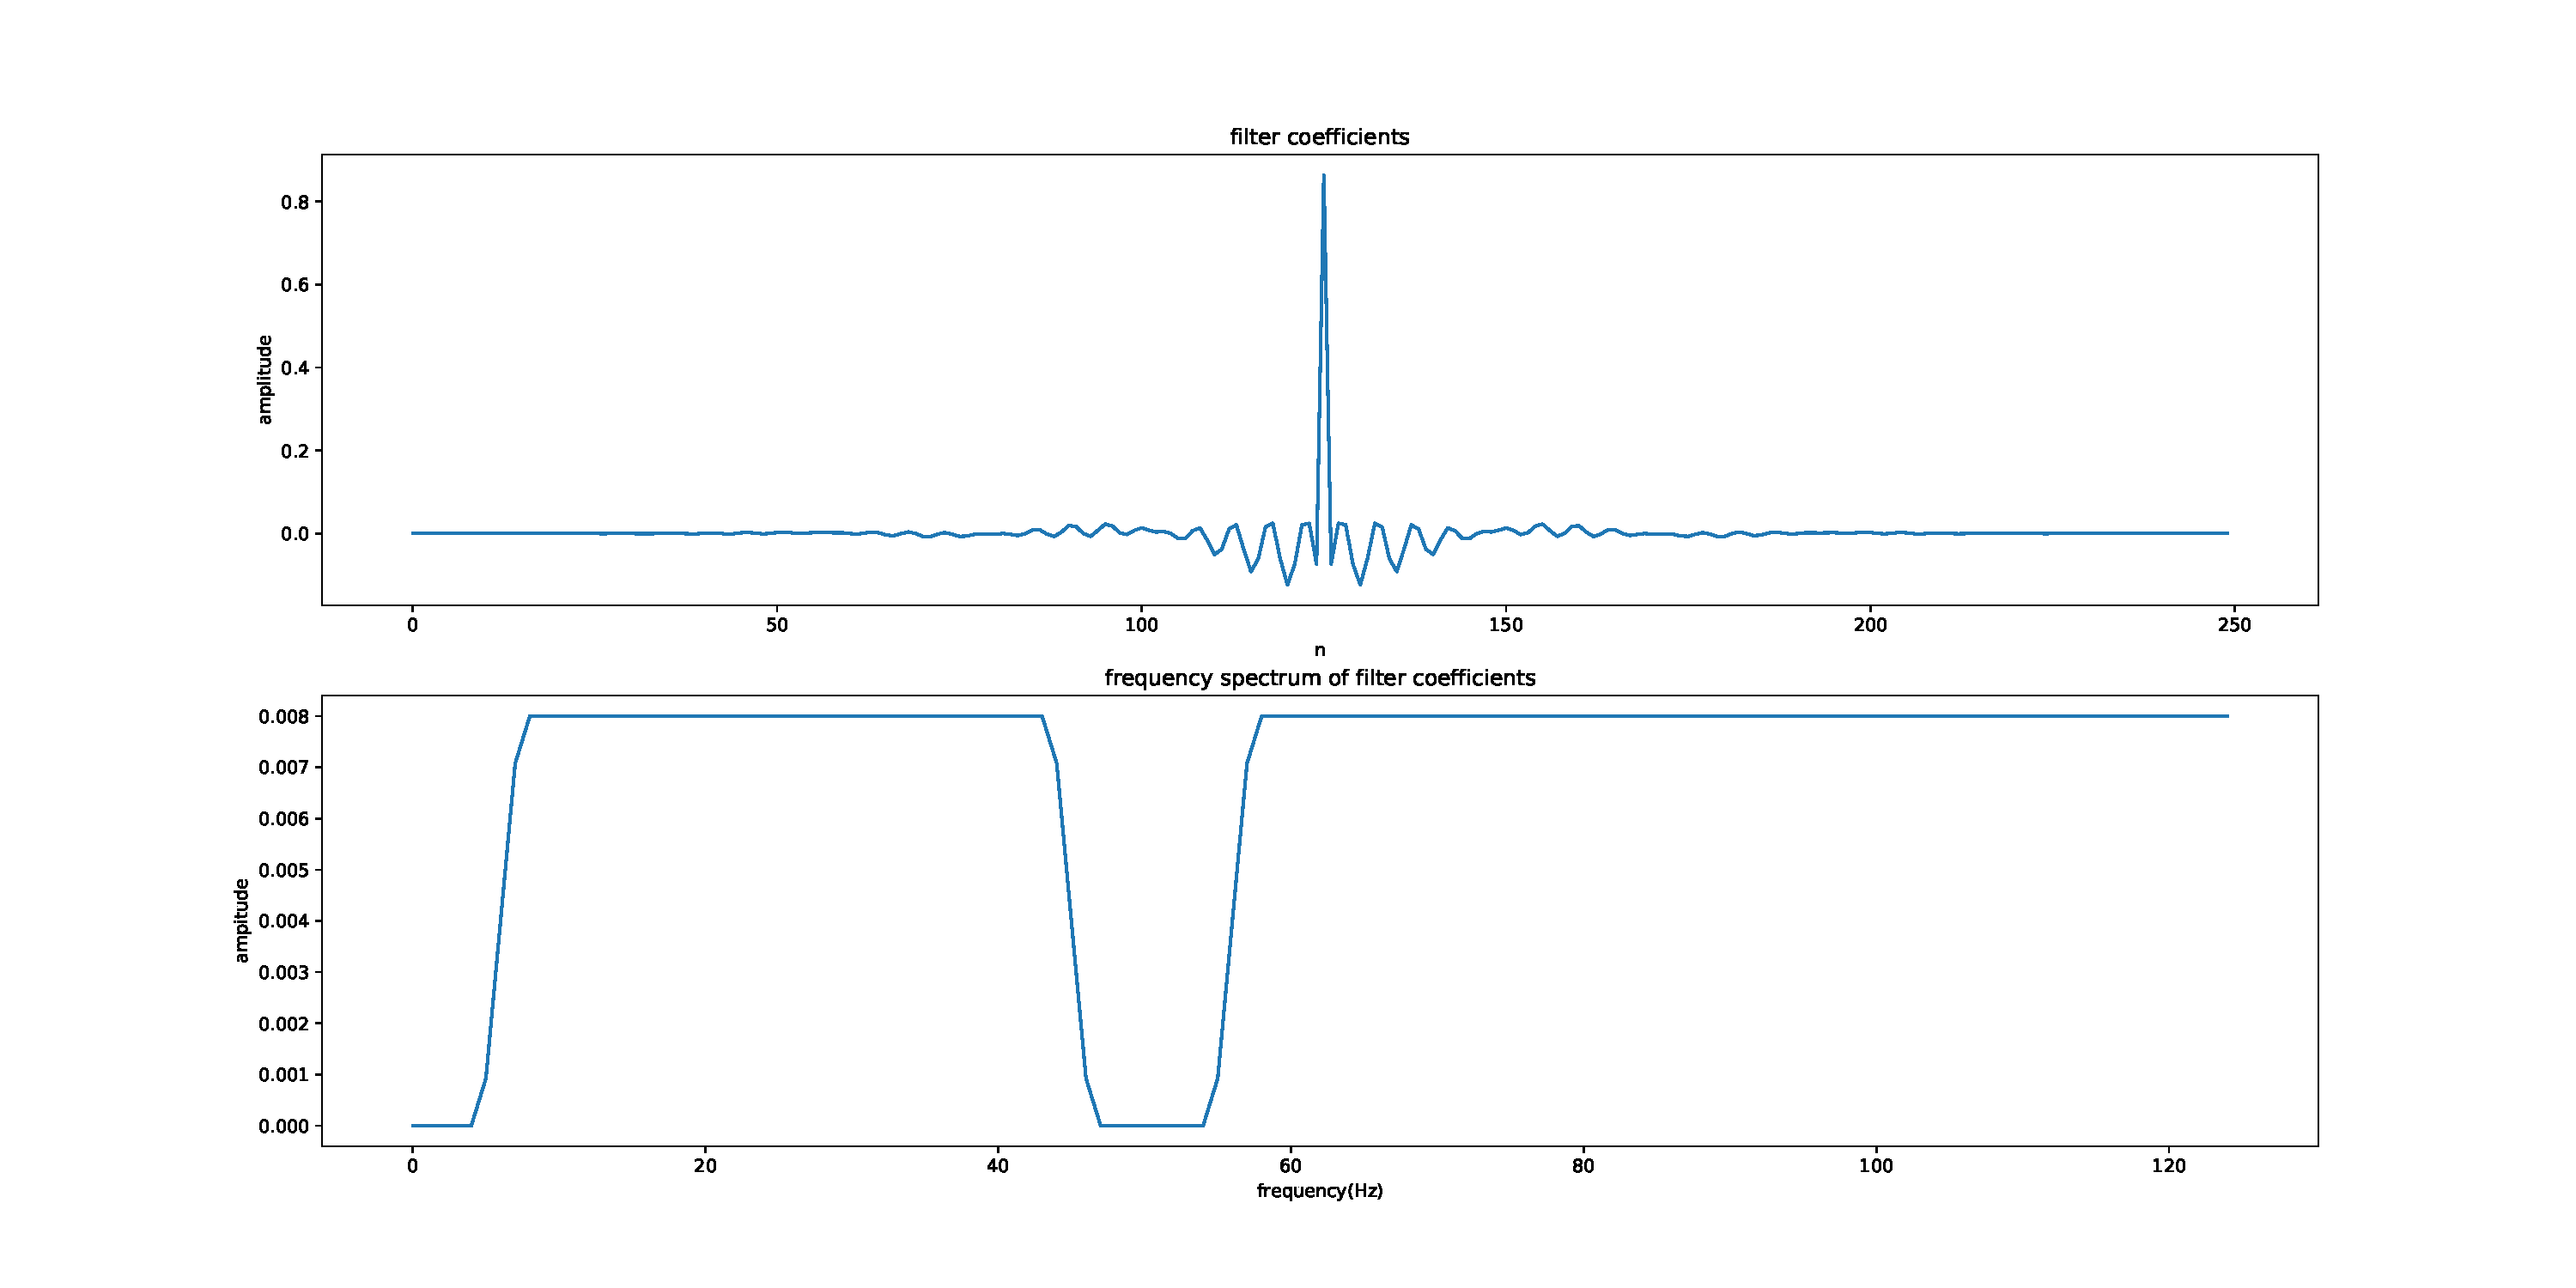
\includegraphics[width=12cm]{../Figures/filterCoefficients.pdf} 
	\caption{filter coefficients}   
	\label{fig_H}
\end{figure}
After we create da fir-filter by this coefficients, for simulating the real time signal, we fed the ECG data into a for loop: 
\begin{lstlisting}[language=Python]
#feed values into filter in real time
fir_filter = fir.FIR_filter(h)
ecgDataFiltered = np.empty(0)
for value in ecgData:
ecgDataFiltered = np.append(ecgDataFiltered, fir_filter.dofilter(value))
\end{lstlisting}
The difference betweent the original siganl and the filtered siganl could be observed in time domain (as shown by \ref{fig_ecgTime}): 
\begin{figure}[H]   
	\centering 
	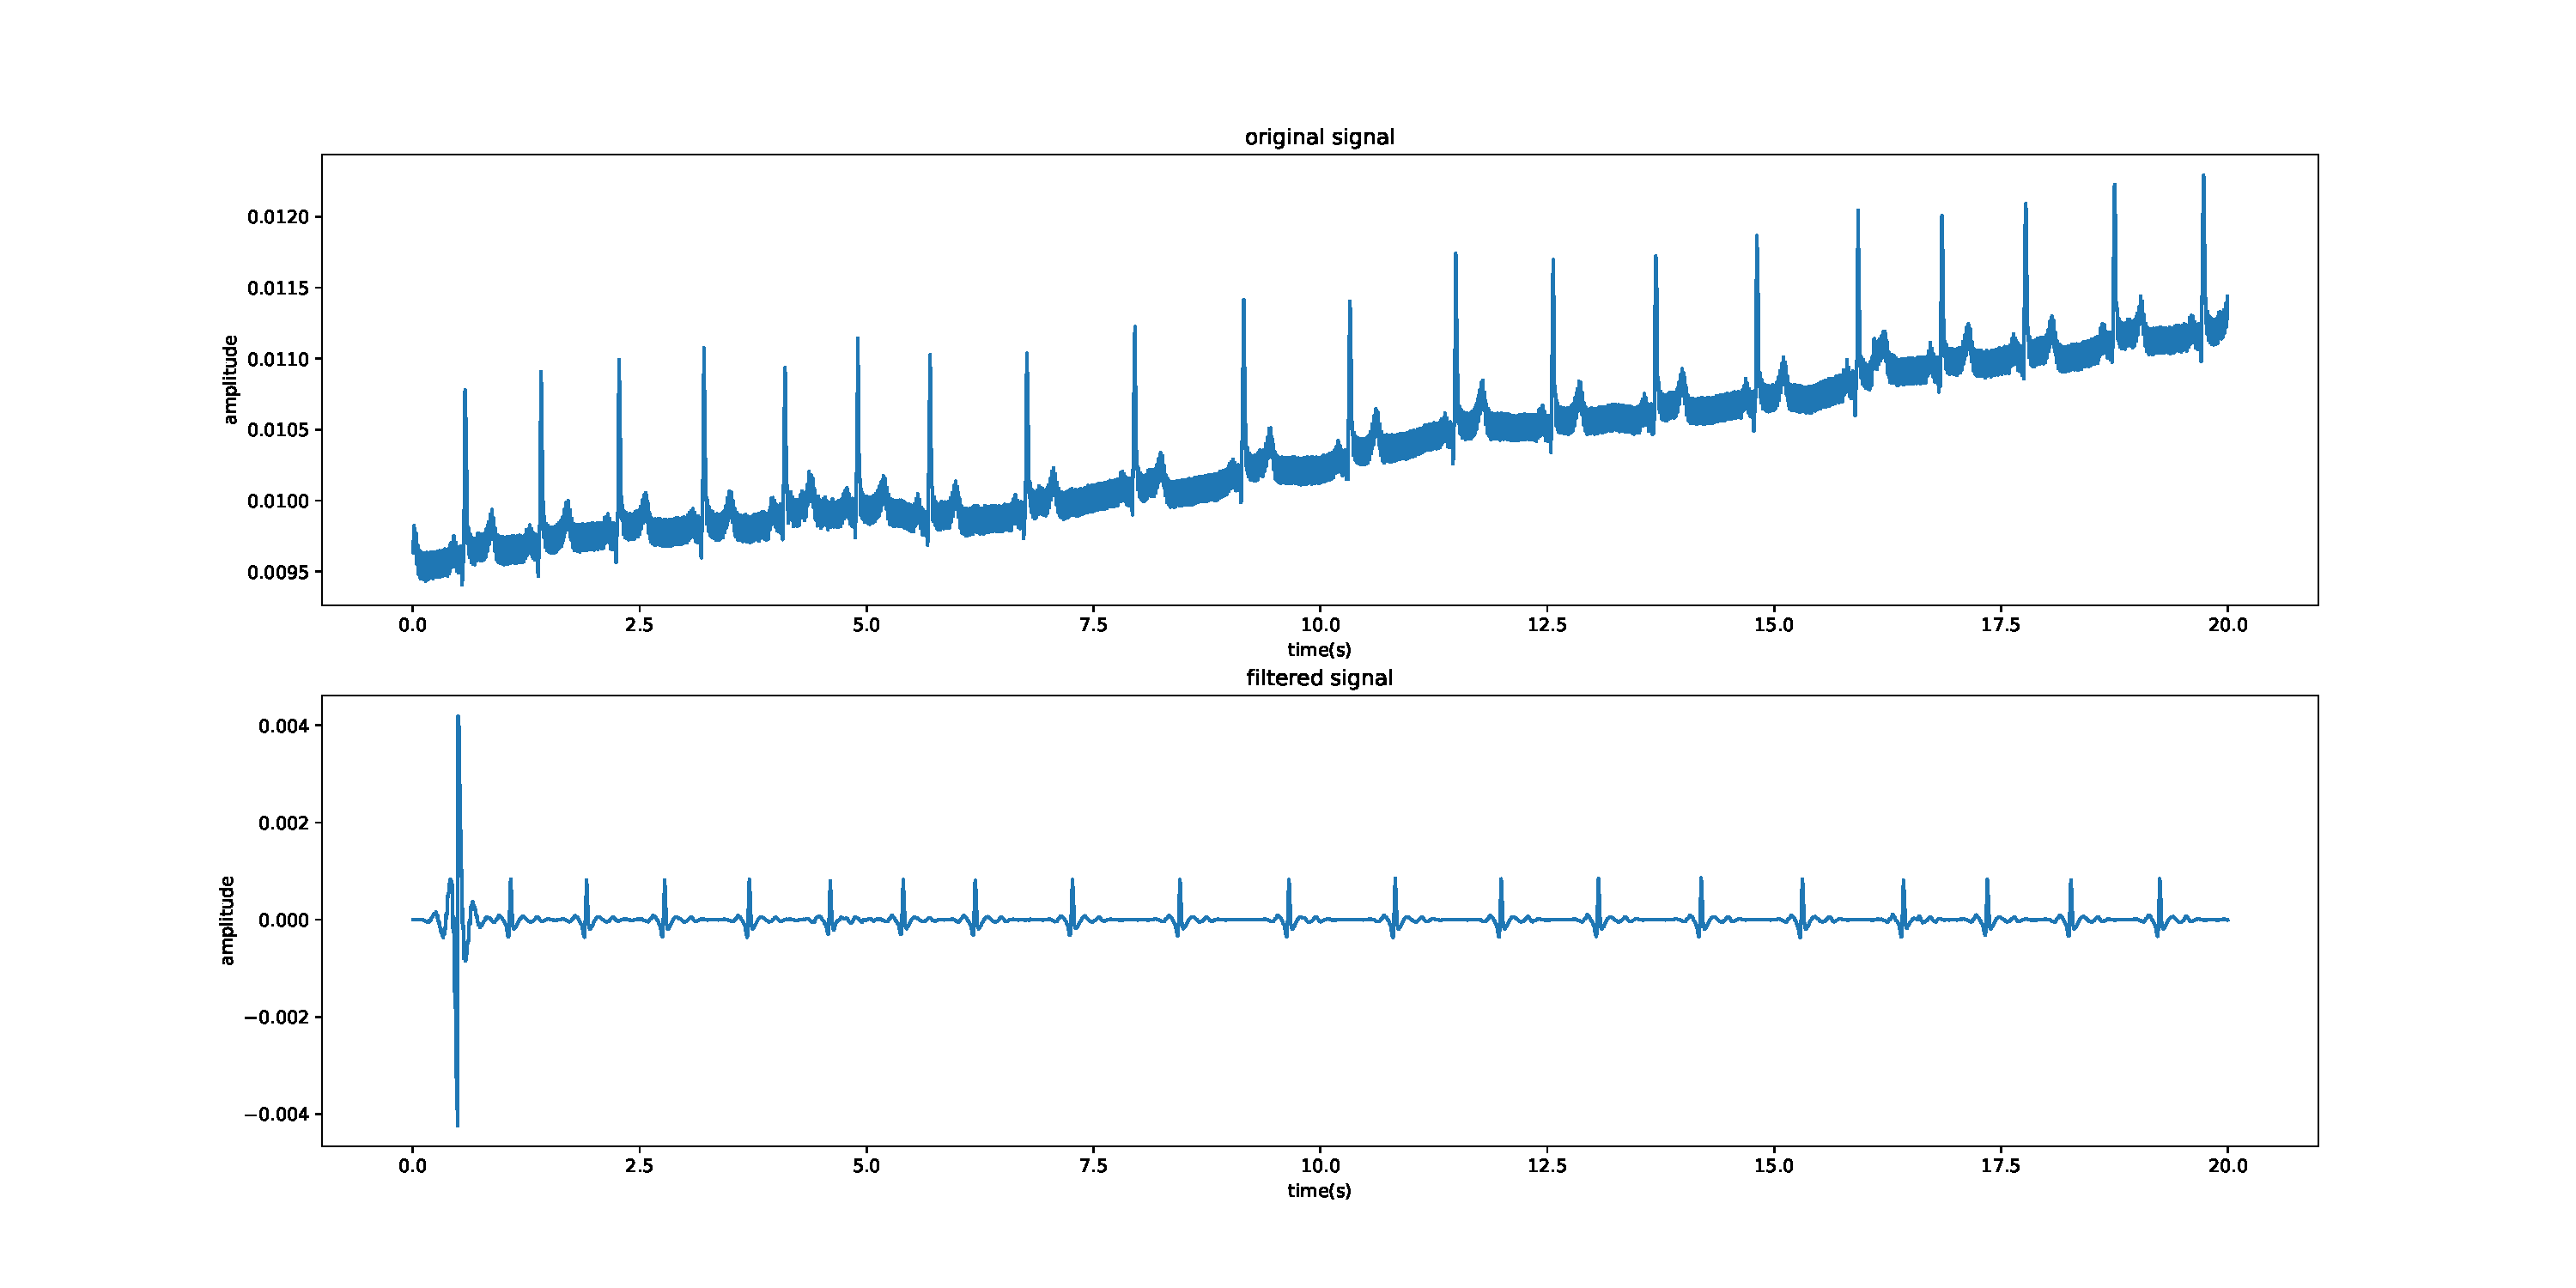
\includegraphics[width=12cm]{../Figures/ecgDataTime.pdf} 
	\caption{ECG data in time domain}   
	\label{fig_ecgTime}
\end{figure}
In frequency domain(as shwon by \ref{fig_ecgFrequency}: 
\begin{figure}[H]   
	\centering 
	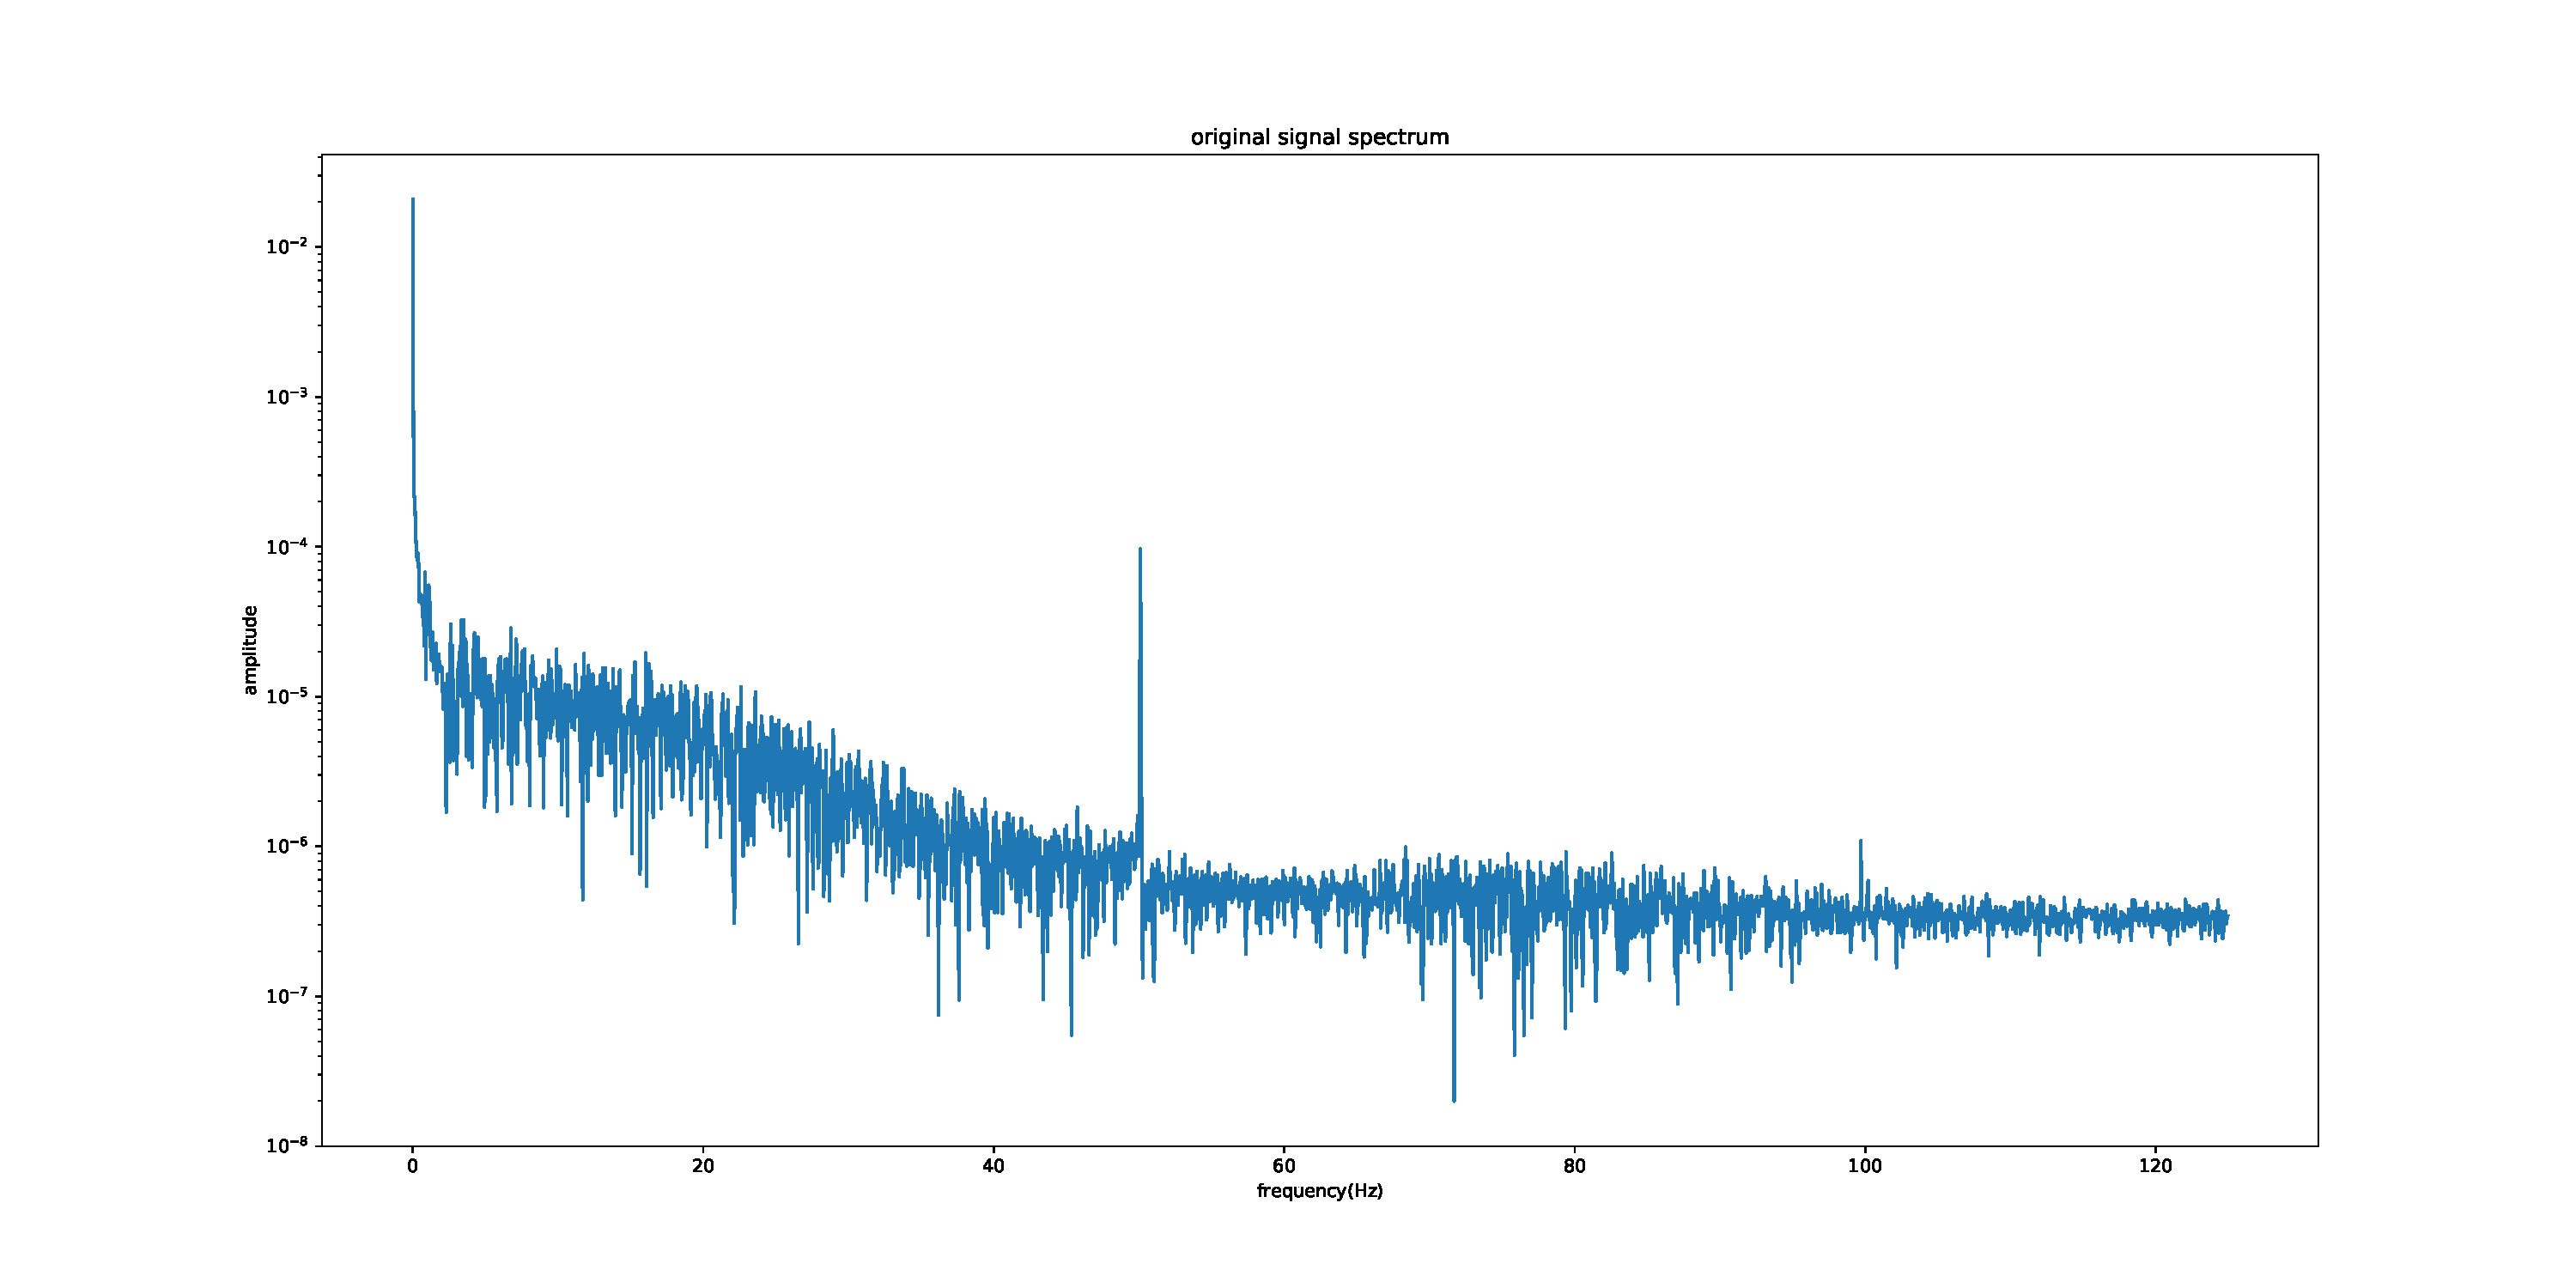
\includegraphics[width=12cm]{../Figures/ecgDataFrequency.pdf} 
	\caption{ECG data in frequency domain}   
	\label{fig_ecgFrequency}
\end{figure}
The PQRST is intact and can be clearly found in figure :
\begin{figure}[H]   
	\centering 
	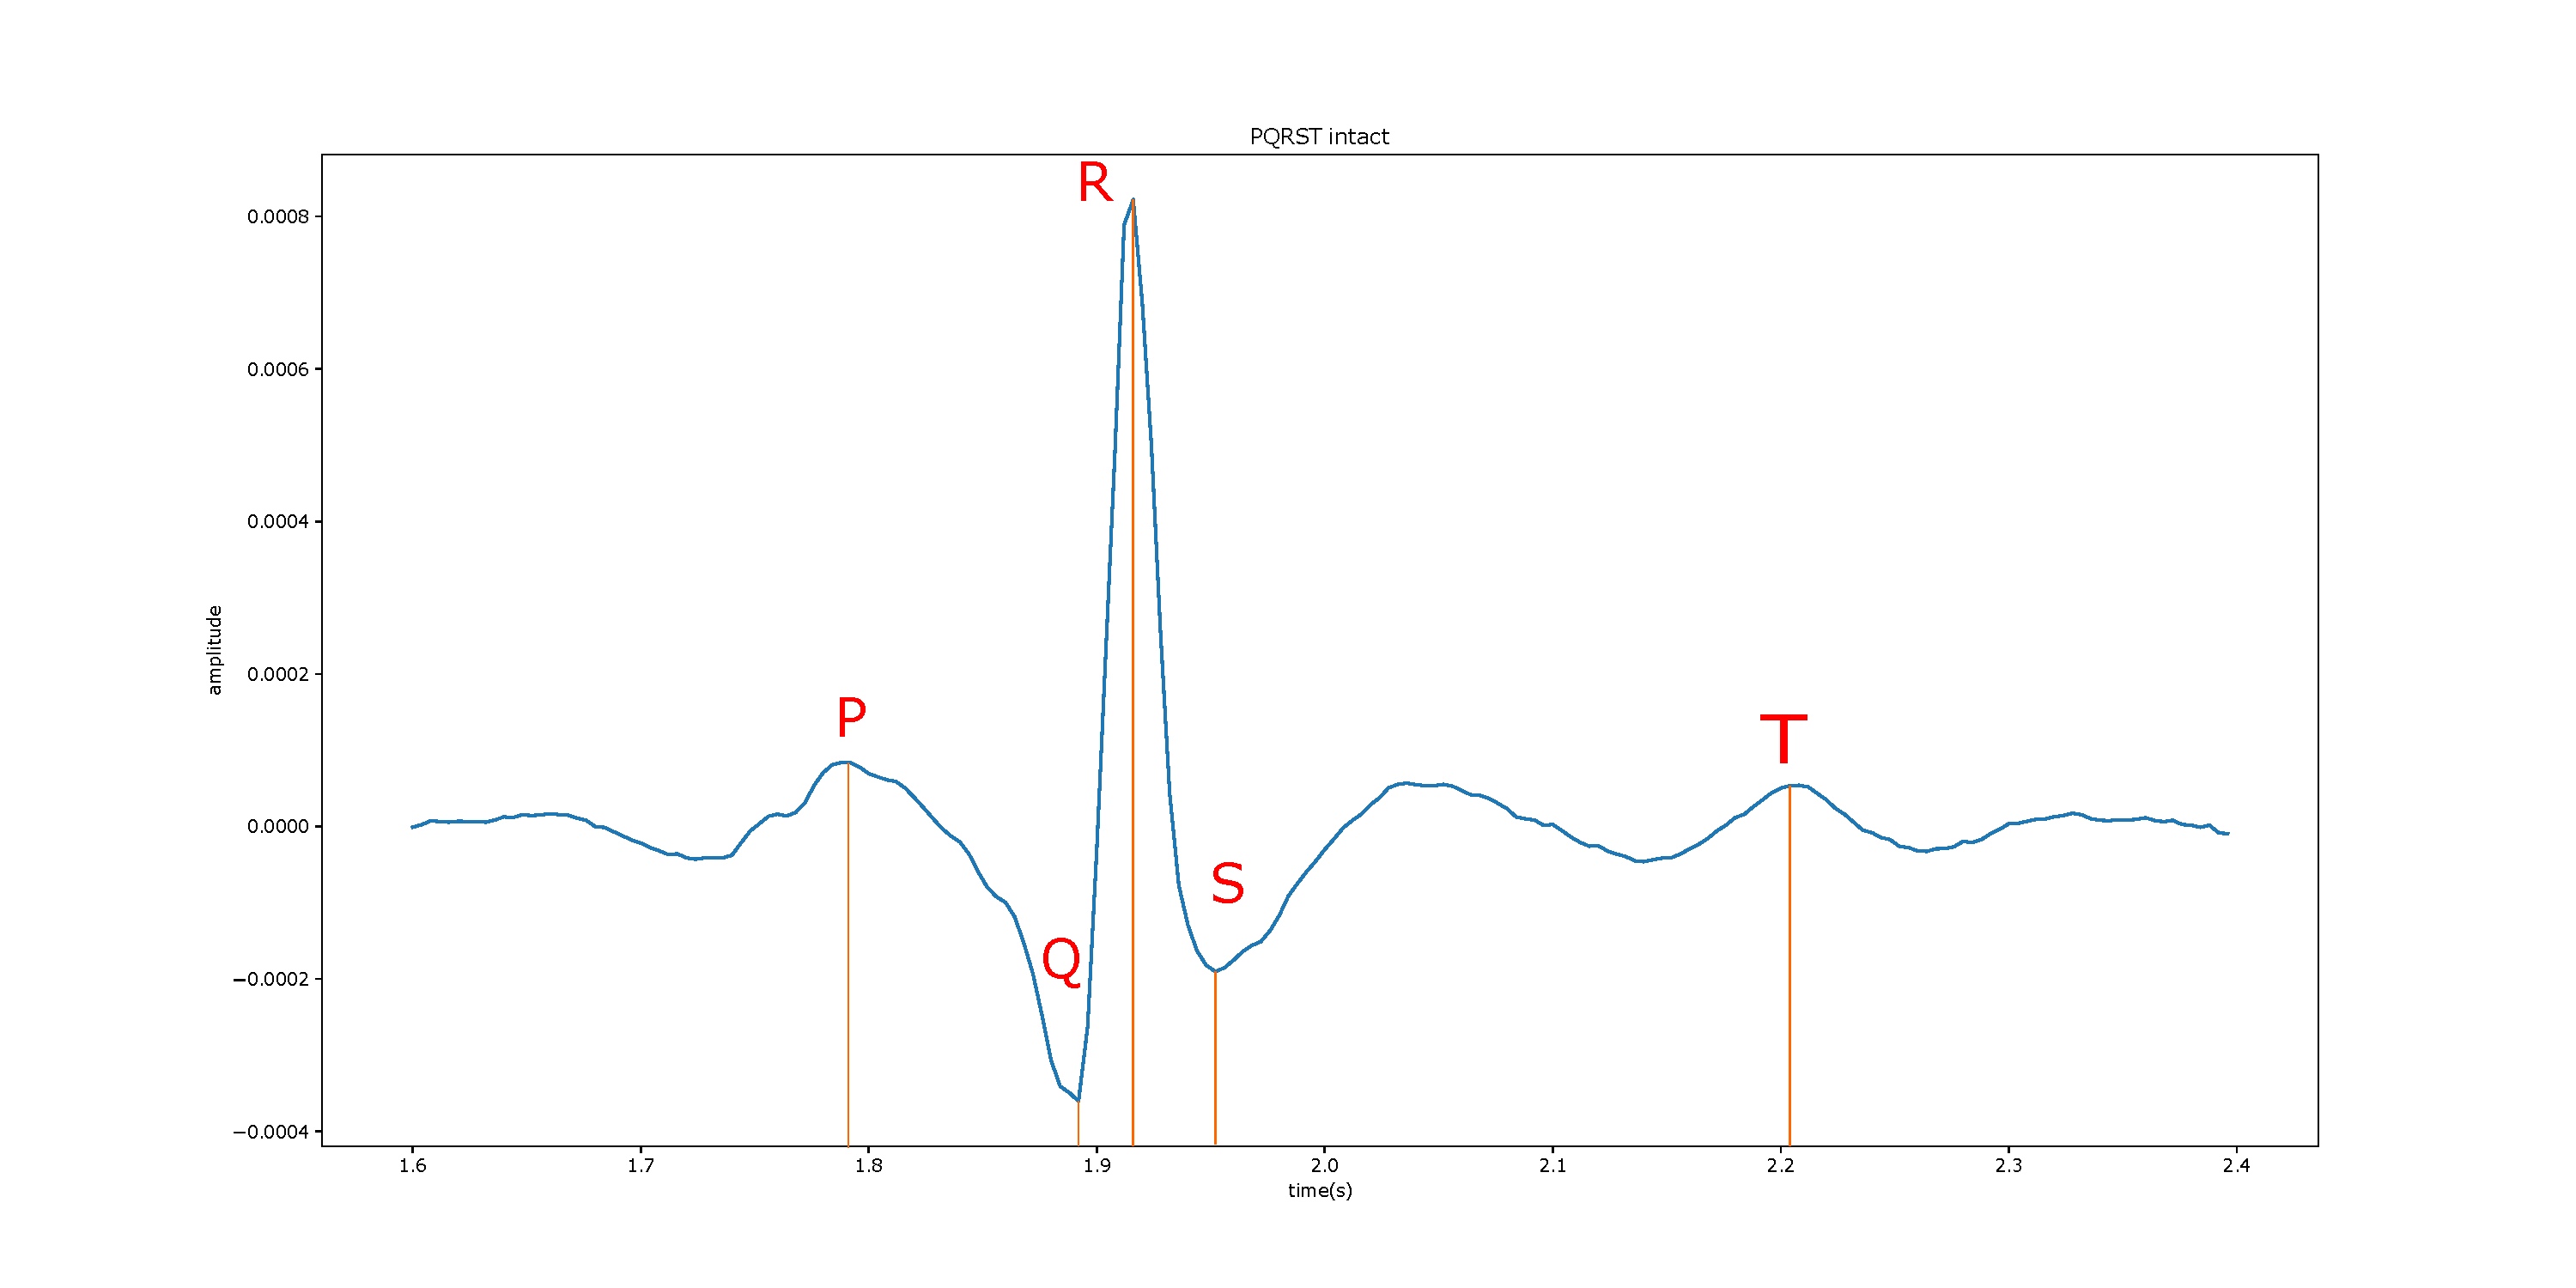
\includegraphics[width=12cm]{../Figures/PQRST.pdf} 
	\caption{PQRST}   
	\label{fig_PQRST}
\end{figure}

\section{Task2}
\subsection{}
To create a template of one single heart beat, we prefiltered the data by the method of Task1 (removing 0~5Hz and 45-55Hz component of the original signal). A template should contain QRST complex. Consequently, we could drive a template as showy by figure \ref{fig_matchCore}
\begin{figure}[H]   
	\centering 
	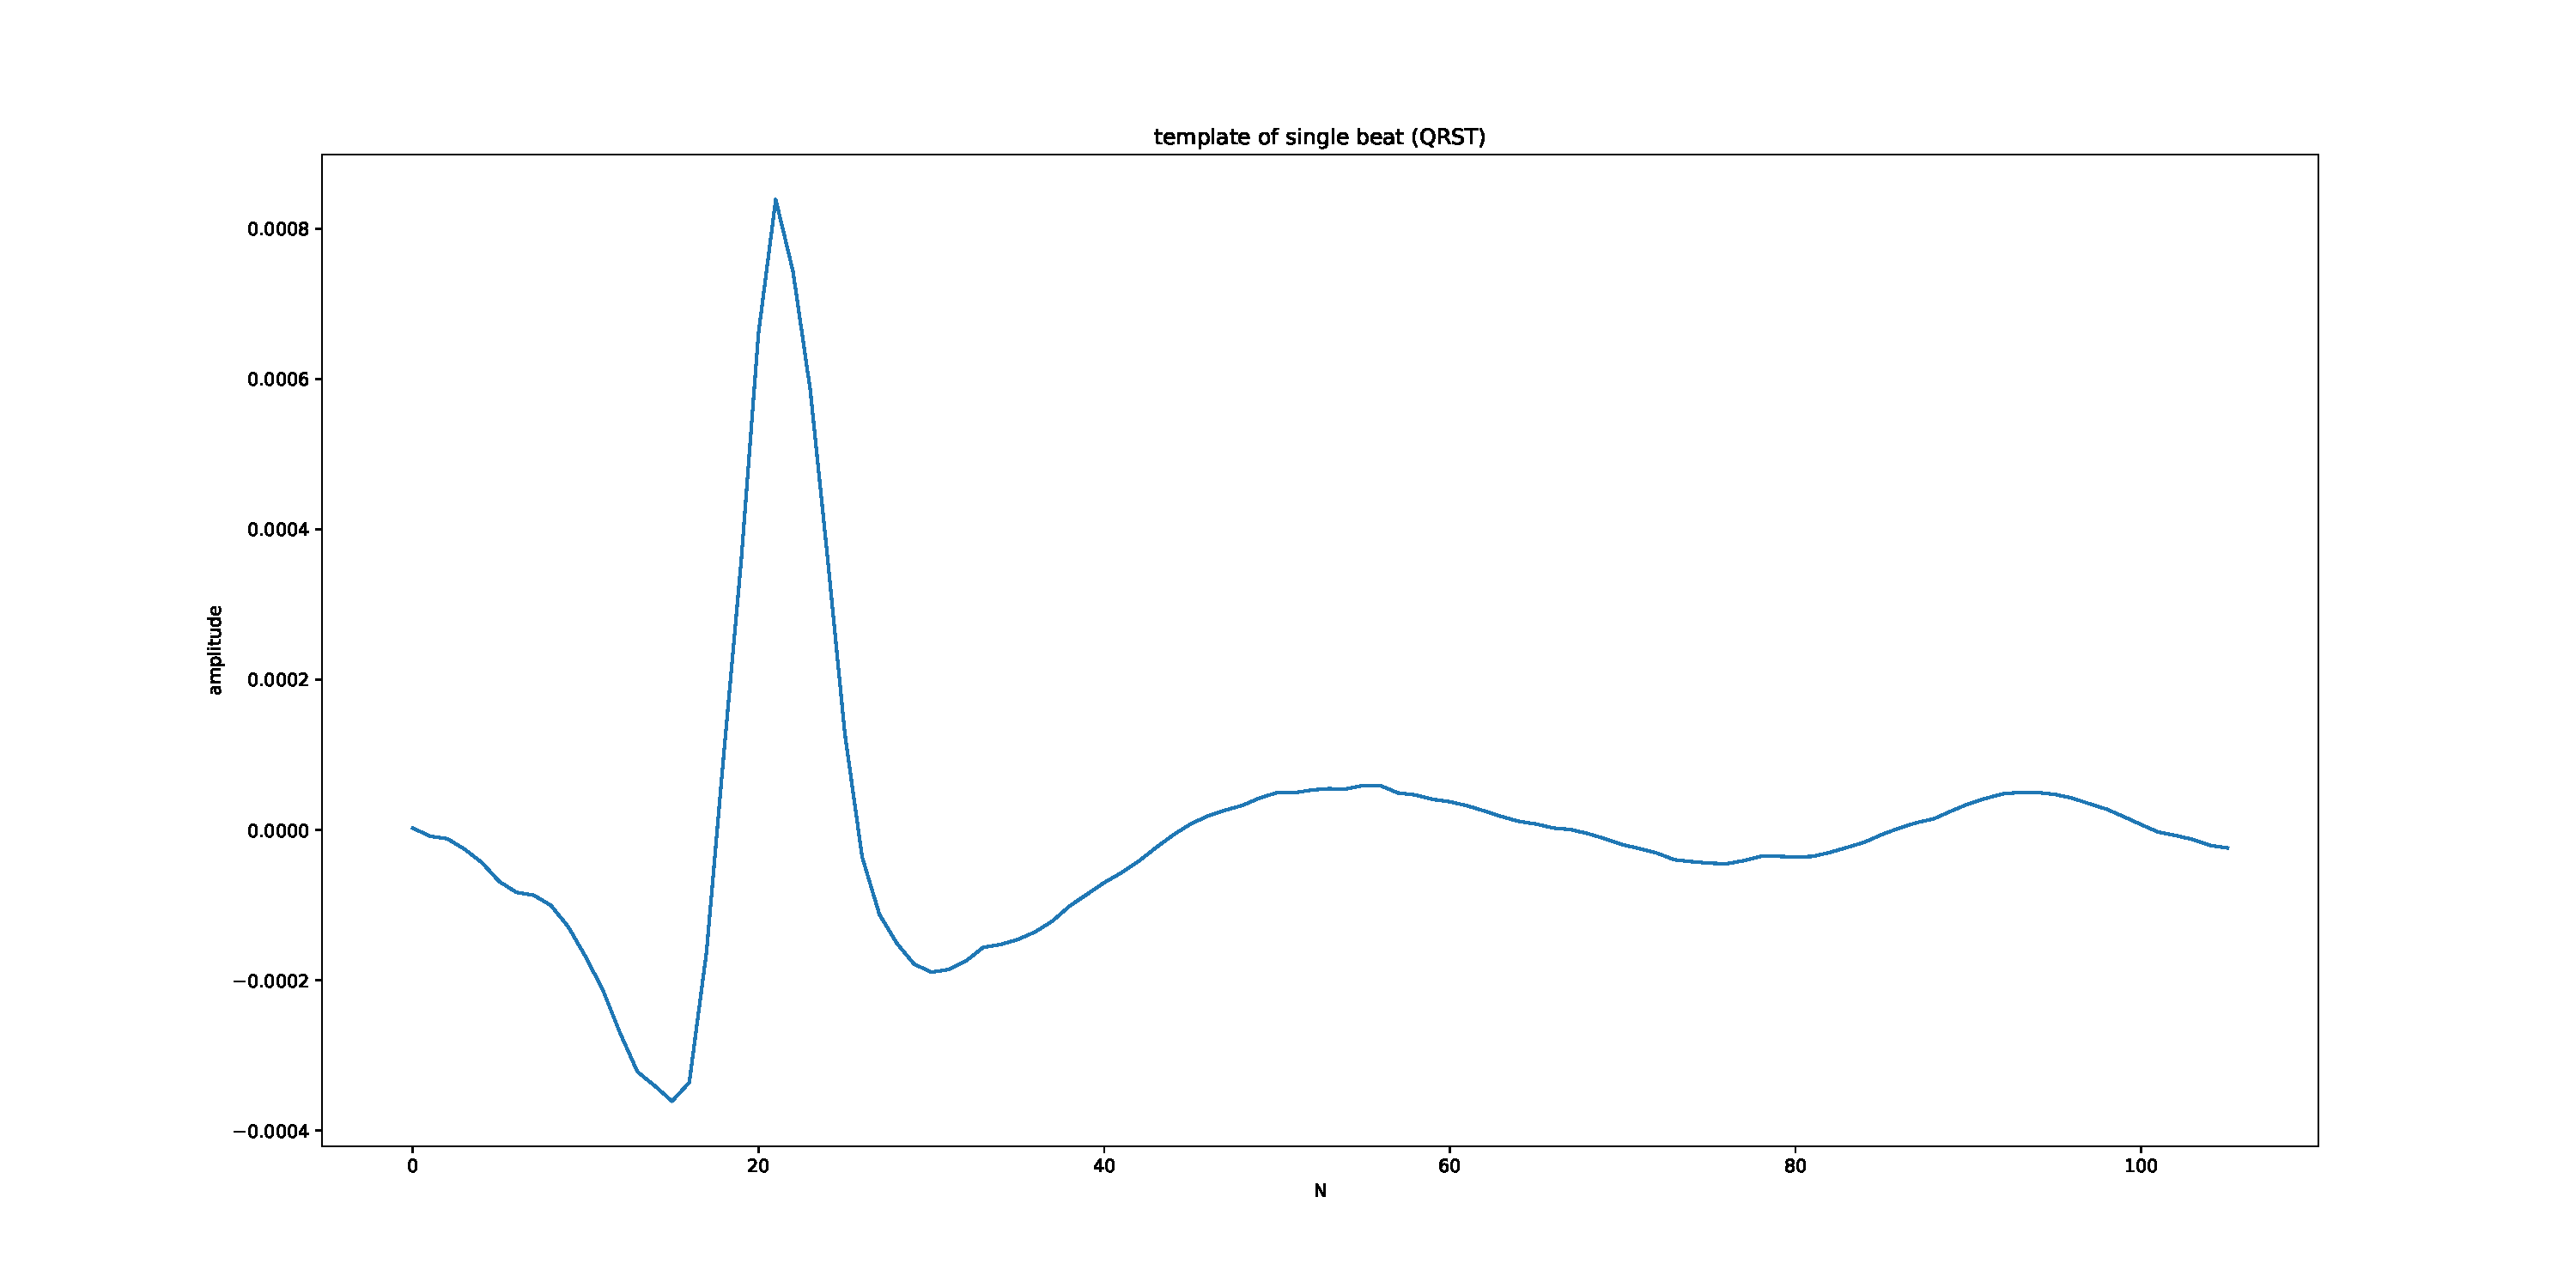
\includegraphics[width=12cm]{../Figures/matchCore.pdf} 
	\caption{single beat of QRST complex}   
	\label{fig_matchCore}
\end{figure}
In order to find the R-peak in real-time processing, we defined a QRST intact when the result of match filter jump exceeds the thresold from low to high.  In code:
\begin{lstlisting}[language=Python]
#when the value exceed the threshold while the previous one didn't
if((matchedDataResult[N-1]>threshold) & (matchedDataResult[N-2] > threshold)):
		peakPosition = np.append(peakPosition, index[0])
\end{lstlisting}
From previous trail and error results, we found one of best threshold:
\begin{lstlisting}[language=Python]
threshold = 0.65e-11
\end{lstlisting}
Than, we fed the signal into our system, which is:
\begin{itemize}
	\item prefilter ever input data
	\item match filter ever input data
	\item check if this data meet the QRST intact found conditions
\end{itemize}
In code:
\begin{lstlisting}[language=Python]
for index, value in np.ndenumerate(ecgData):
		prefilteredData = preFilter1.dofilter(value)
		#record prefilter result
		preFilterResult = np.append(preFilterResult, prefilteredData)
		#record matchfilter result
		matchedData = matchedFilter1.dofilter(prefilteredData)**2 #reduce S/N ratio
		matchedDataResult = np.append(matchedDataResult, matchedData)
		
		#define threshold
		threshold = 0.65e-11
		N = len(matchedDataResult)
		#when the value exceeded the threshold while the previous one didn't
		if((matchedDataResult[N-1]>threshold) & (matchedDataResult[N-2] > threshold)):
		peakPosition = np.append(peakPosition, index[0])
\end{lstlisting}
And the result of match filter is shown by figure\ref{fig_matchResult}:
\begin{figure}[H]   
	\centering 
	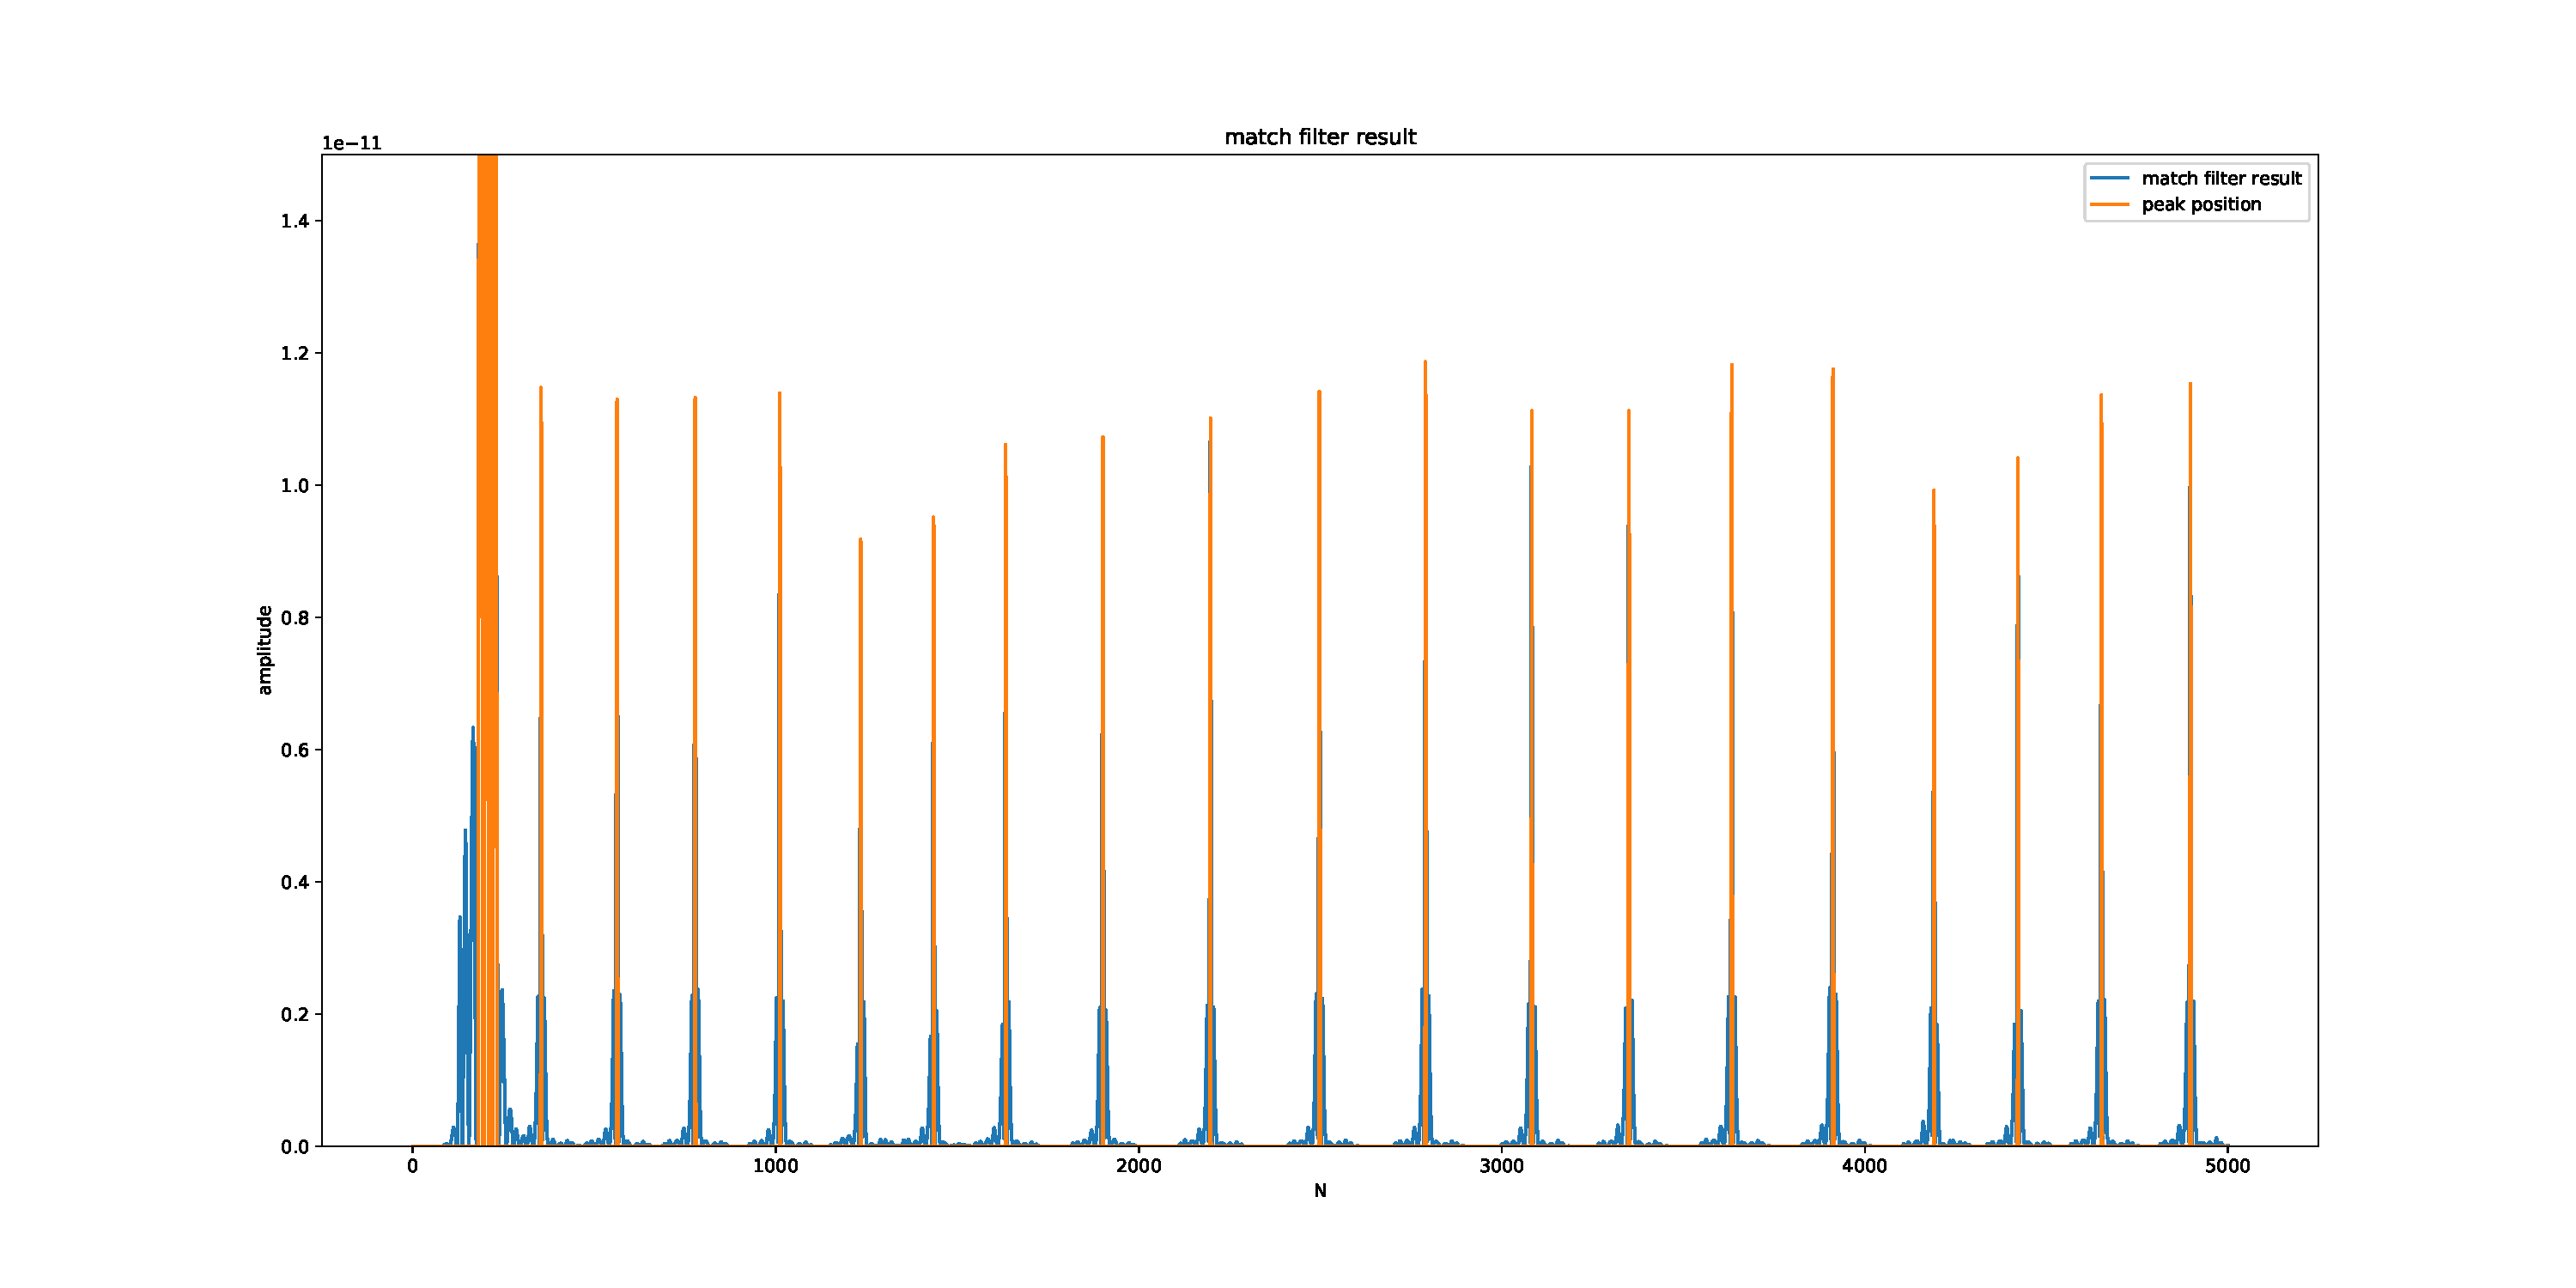
\includegraphics[width=12cm]{../Figures/matchResult.pdf} 
	\caption{the match filter result and the found peaks} 
	\label{fig_matchResult}
\end{figure}
\subsection{}
Heart rate can be calculated by the time gap between every heart beat (R-peak). Specifically:
\begin{lstlisting}[language=Python]
heartRate =60//(N*(1/Fs))
\end{lstlisting}
Where N is the number of sample points between each detected heart beat\\
Besides, for removing wrong detections, we limited the minimum interval to 100 sampling points. When coding,  an IF statement has been implemented for this operator
\begin{lstlisting}[language=Python]
if(N>Nlimited):
\end{lstlisting}
Consequently, when we implemeted the heart rate detect funtion for each input data, it is similar to the R-peak detecting at the beginning:
\begin{lstlisting}[language=Python]
#do prefilter
preFltValue = preFilter.dofilter(value)
#do match filter
matchedValue = matchedFilter.dofilter(preFltValue)
#increase S/N ratio
matchedValue *= matchedValue
\end{lstlisting}
Than we recorded  each sampling point during the gap between each heat beat:
\begin{lstlisting}[language=Python]
#recordding gap
template = np.append(template, matchedValue)
\end{lstlisting}
Once a heart beat had been detected, we calculate the new value of heartbeats rate and restart calculating the gap:
\begin{lstlisting}[language=Python]
N = len(template)
if(N>Nlimited):
		if((template[N-1]>threshold)&(template[N-2]<threshold)):
				#calculate the heartRate
				heartRate =60//(N*(1/Fs))
				#calculate the time when beat occur
				time = index[0]*(1/Fs)
				print("in",round(time, 2),"s:", heartRate, "Bpm")
				heartRateResult = np.append(heartRateResult, heartRate)
				
#clear template
template = np.empty(0)
\end{lstlisting}
The final output of heartbeat in real-time system is shown by figure\ref{fig_heartRate}
\begin{figure}[H]   
	\centering 
	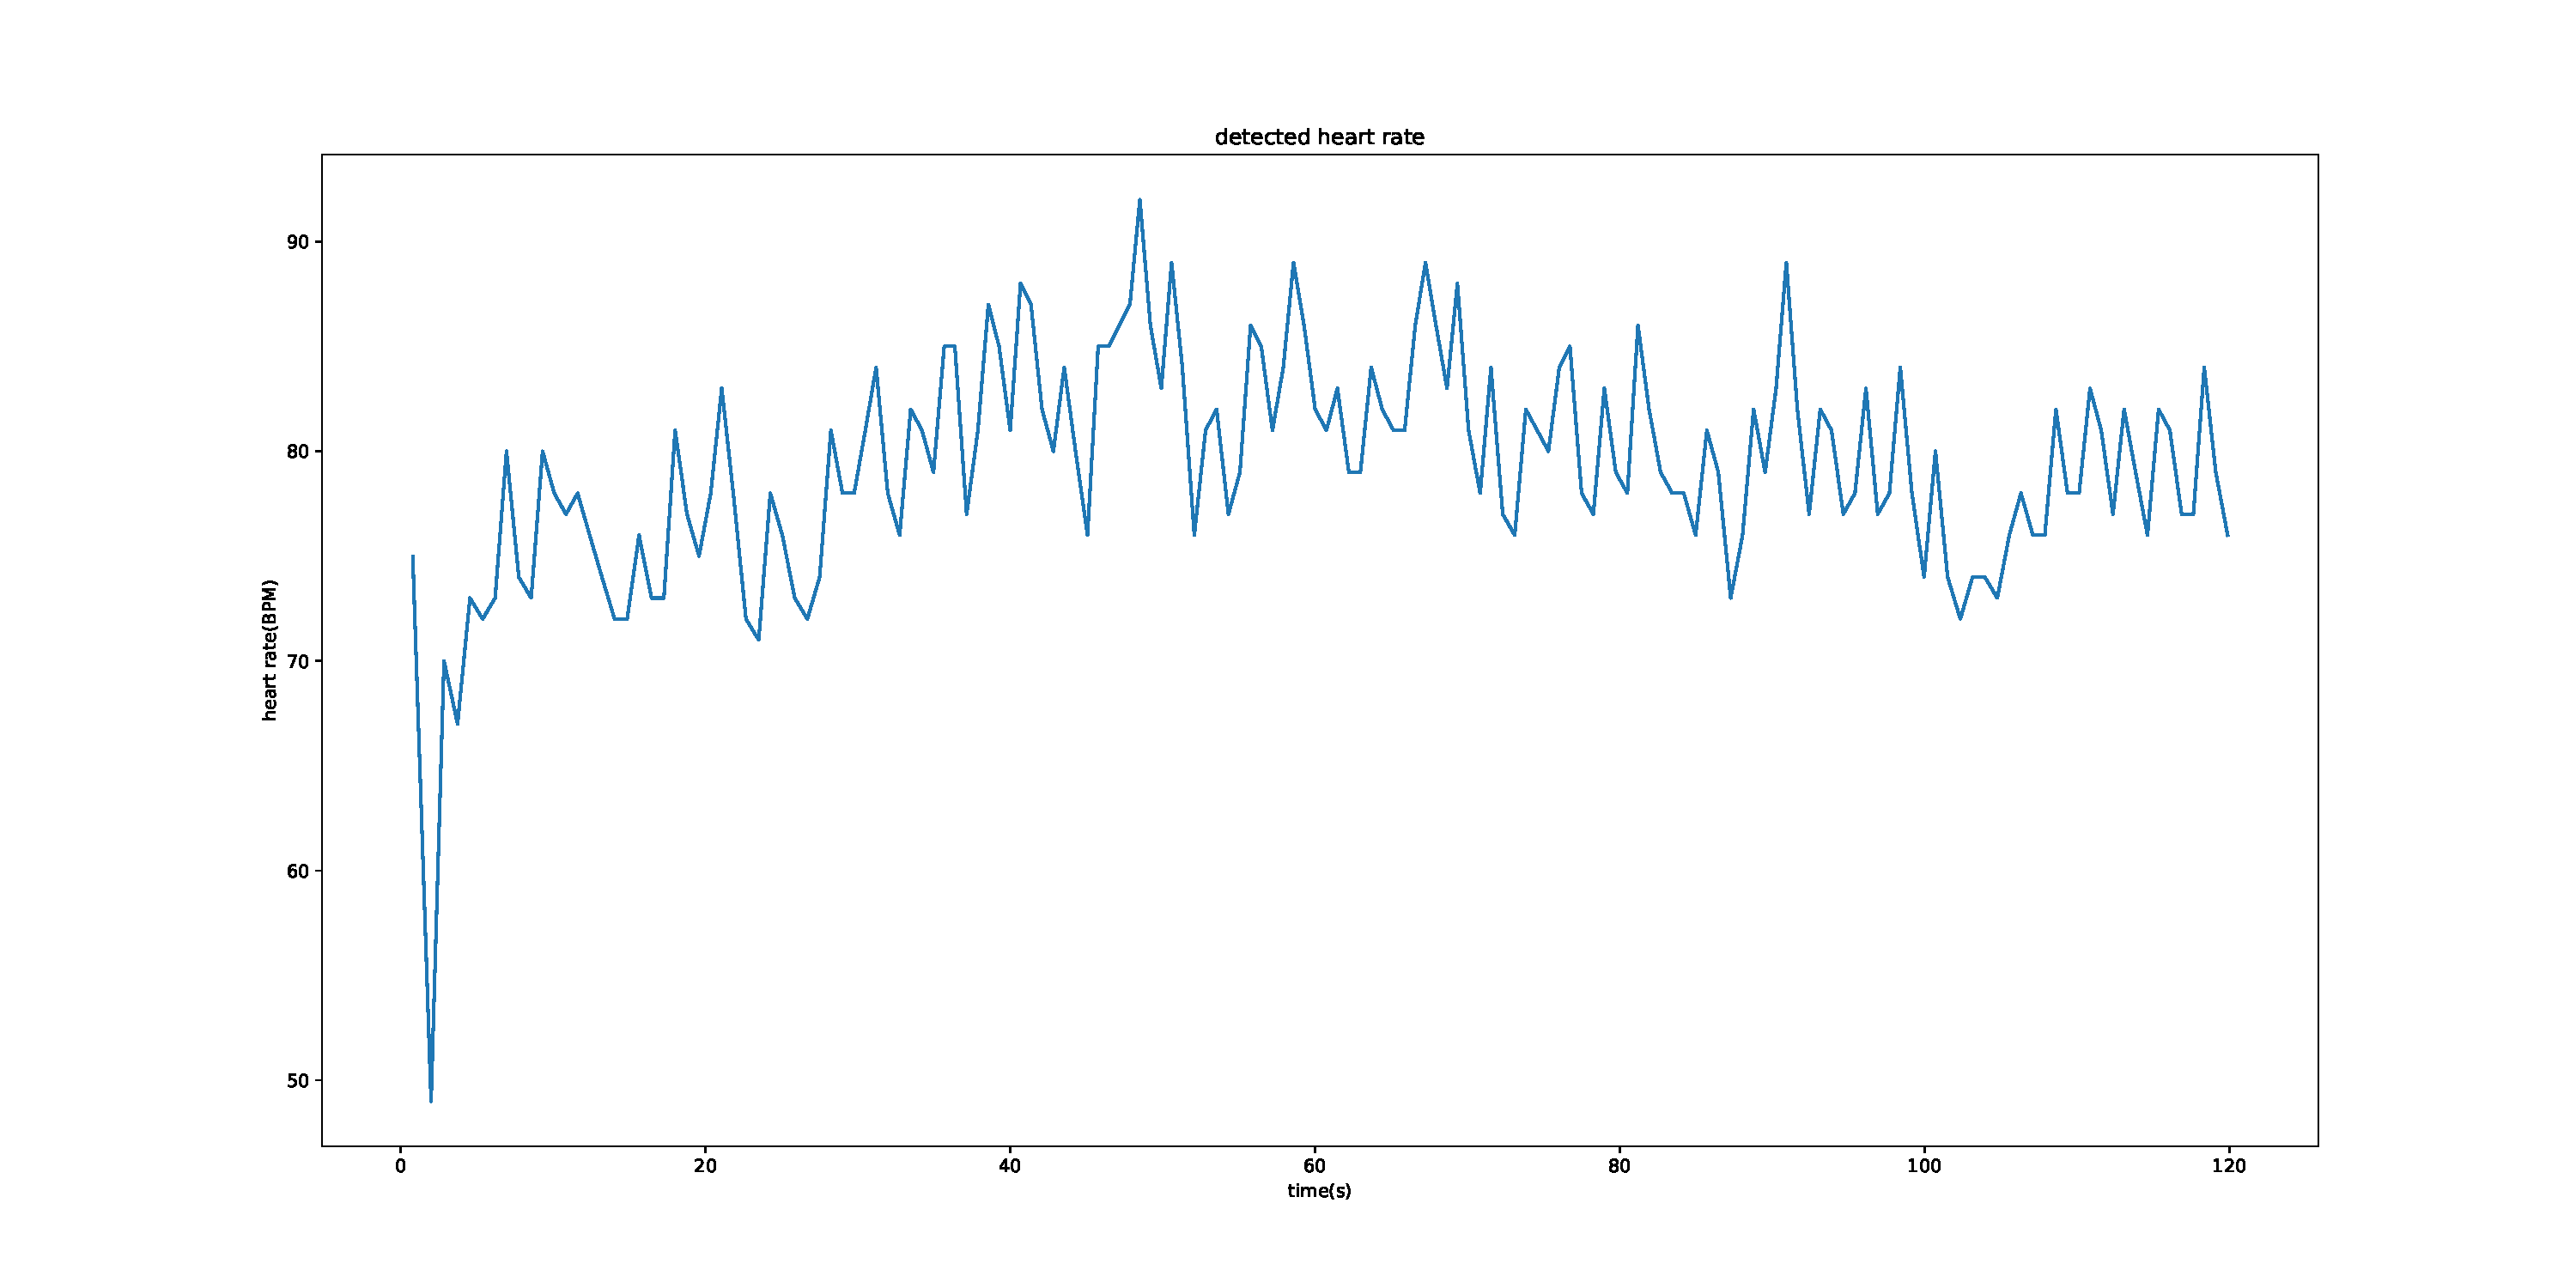
\includegraphics[width=12cm]{../Figures/heartRate.pdf} 
	\caption{the match filter result and the found peaks} 
	\label{fig_heartRate}
\end{figure}
In command line:
\begin{lstlisting}
in 0.79 s: 75.0 Bpm
in 2.0 s: 49.0 Bpm
in 2.84 s: 70.0 Bpm
in 3.73 s: 67.0 Bpm
in 4.55 s: 73.0 Bpm
in 5.38 s: 72.0 Bpm
in 6.2 s: 73.0 Bpm
in 6.94 s: 80.0 Bpm
in 7.75 s: 74.0 Bpm
in 8.56 s: 73.0 Bpm
in 9.31 s: 80.0 Bpm
in 10.08 s: 78.0 Bpm
in 10.85 s: 77.0 Bpm
in 11.61 s: 78.0 Bpm
in 12.4 s: 76.0 Bpm
in 13.21 s: 74.0 Bpm
in 14.04 s: 72.0 Bpm
in 14.86 s: 72.0 Bpm
in 15.64 s: 76.0 Bpm
in 16.46 s: 73.0 Bpm
in 17.27 s: 73.0 Bpm
in 18.01 s: 81.0 Bpm
in 18.79 s: 77.0 Bpm
in 19.58 s: 75.0 Bpm
in 20.35 s: 78.0 Bpm
in 21.07 s: 83.0 Bpm
in 21.83 s: 78.0 Bpm
in 22.66 s: 72.0 Bpm
in 23.5 s: 71.0 Bpm
in 24.26 s: 78.0 Bpm
in 25.04 s: 76.0 Bpm
in 25.86 s: 73.0 Bpm
in 26.69 s: 72.0 Bpm
in 27.5 s: 74.0 Bpm
in 28.23 s: 81.0 Bpm
in 28.99 s: 78.0 Bpm
in 29.76 s: 78.0 Bpm
in 30.49 s: 81.0 Bpm
in 31.2 s: 84.0 Bpm
in 31.96 s: 78.0 Bpm
in 32.74 s: 76.0 Bpm
in 33.47 s: 82.0 Bpm
in 34.21 s: 81.0 Bpm
in 34.96 s: 79.0 Bpm
in 35.67 s: 85.0 Bpm
in 36.37 s: 85.0 Bpm
in 37.14 s: 77.0 Bpm
in 37.88 s: 81.0 Bpm
in 38.57 s: 87.0 Bpm
in 39.27 s: 85.0 Bpm
in 40.0 s: 81.0 Bpm
in 40.68 s: 88.0 Bpm
in 41.36 s: 87.0 Bpm
in 42.09 s: 82.0 Bpm
in 42.83 s: 80.0 Bpm
in 43.54 s: 84.0 Bpm
in 44.29 s: 80.0 Bpm
in 45.07 s: 76.0 Bpm
in 45.77 s: 85.0 Bpm
in 46.48 s: 85.0 Bpm
in 47.17 s: 86.0 Bpm
in 47.86 s: 87.0 Bpm
in 48.51 s: 92.0 Bpm
in 49.2 s: 86.0 Bpm
in 49.92 s: 83.0 Bpm
in 50.59 s: 89.0 Bpm
in 51.3 s: 84.0 Bpm
in 52.08 s: 76.0 Bpm
in 52.82 s: 81.0 Bpm
in 53.54 s: 82.0 Bpm
in 54.32 s: 77.0 Bpm
in 55.08 s: 79.0 Bpm
in 55.77 s: 86.0 Bpm
in 56.48 s: 85.0 Bpm
in 57.21 s: 81.0 Bpm
in 57.92 s: 84.0 Bpm
in 58.59 s: 89.0 Bpm
in 59.28 s: 86.0 Bpm
in 60.01 s: 82.0 Bpm
in 60.75 s: 81.0 Bpm
in 61.47 s: 83.0 Bpm
in 62.22 s: 79.0 Bpm
in 62.98 s: 79.0 Bpm
in 63.69 s: 84.0 Bpm
in 64.41 s: 82.0 Bpm
in 65.15 s: 81.0 Bpm
in 65.88 s: 81.0 Bpm
in 66.58 s: 86.0 Bpm
in 67.25 s: 89.0 Bpm
in 67.94 s: 86.0 Bpm
in 68.66 s: 83.0 Bpm
in 69.34 s: 88.0 Bpm
in 70.08 s: 81.0 Bpm
in 70.84 s: 78.0 Bpm
in 71.55 s: 84.0 Bpm
in 72.32 s: 77.0 Bpm
in 73.11 s: 76.0 Bpm
in 73.84 s: 82.0 Bpm
in 74.57 s: 81.0 Bpm
in 75.32 s: 80.0 Bpm
in 76.03 s: 84.0 Bpm
in 76.73 s: 85.0 Bpm
in 77.5 s: 78.0 Bpm
in 78.27 s: 77.0 Bpm
in 78.99 s: 83.0 Bpm
in 79.74 s: 79.0 Bpm
in 80.5 s: 78.0 Bpm
in 81.2 s: 86.0 Bpm
in 81.92 s: 82.0 Bpm
in 82.68 s: 79.0 Bpm
in 83.44 s: 78.0 Bpm
in 84.2 s: 78.0 Bpm
in 84.98 s: 76.0 Bpm
in 85.72 s: 81.0 Bpm
in 86.47 s: 79.0 Bpm
in 87.28 s: 73.0 Bpm
in 88.06 s: 76.0 Bpm
in 88.78 s: 82.0 Bpm
in 89.54 s: 79.0 Bpm
in 90.26 s: 83.0 Bpm
in 90.93 s: 89.0 Bpm
in 91.66 s: 82.0 Bpm
in 92.43 s: 77.0 Bpm
in 93.16 s: 82.0 Bpm
in 93.9 s: 81.0 Bpm
in 94.67 s: 77.0 Bpm
in 95.44 s: 78.0 Bpm
in 96.16 s: 83.0 Bpm
in 96.93 s: 77.0 Bpm
in 97.7 s: 78.0 Bpm
in 98.41 s: 84.0 Bpm
in 99.17 s: 78.0 Bpm
in 99.97 s: 74.0 Bpm
in 100.72 s: 80.0 Bpm
in 101.52 s: 74.0 Bpm
in 102.35 s: 72.0 Bpm
in 103.15 s: 74.0 Bpm
in 103.96 s: 74.0 Bpm
in 104.78 s: 73.0 Bpm
in 105.56 s: 76.0 Bpm
in 106.33 s: 78.0 Bpm
in 107.11 s: 76.0 Bpm
in 107.9 s: 76.0 Bpm
in 108.62 s: 82.0 Bpm
in 109.38 s: 78.0 Bpm
in 110.14 s: 78.0 Bpm
in 110.86 s: 83.0 Bpm
in 111.6 s: 81.0 Bpm
in 112.37 s: 77.0 Bpm
in 113.1 s: 82.0 Bpm
in 113.85 s: 79.0 Bpm
in 114.63 s: 76.0 Bpm
in 115.36 s: 82.0 Bpm
in 116.1 s: 81.0 Bpm
in 116.87 s: 77.0 Bpm
in 117.64 s: 77.0 Bpm
in 118.36 s: 84.0 Bpm
in 119.11 s: 79.0 Bpm
in 119.89 s: 76.0 Bpm
\end{lstlisting}

\clearpage

\section{Appendix}
\subsection{hr-detect.py}
\lstinputlisting[language=Python]{\string"../hr_detect.py"}
\subsection{ecg-filter.py}
\lstinputlisting[language=Python]{\string"../ecg_filter.py"}
\subsection{fir-filter.py}
\lstinputlisting[language=Python]{\string"../fir_filter.py"}

\end{document}

